\documentclass[12pt,a4paper]{article}
\usepackage[utf8]{inputenc}
\usepackage{graphicx}
% Document config
\usepackage[letterpaper, margin=1in]{geometry}
\usepackage[spanish]{babel}
\usepackage[utf8]{inputenc}
\usepackage{tikz}
\usepackage{hyperref}
\usepackage{minted,xcolor}
\usemintedstyle{tango}
\usepackage{color}
\usepackage{xcolor}
\usepackage{float}
\usepackage{tcolorbox}
\usepackage[nottoc]{tocbibind}
\usepackage{graphicx}
\usepackage{listings}
\usepackage{lineno}
\usepackage{fancyvrb}
\usepackage{minted}
\usepackage[utf8]{inputenc}
\usepackage{pdfpages} %para importar paginas de un pdf
\usepackage{multirow}
\addto\captionsspanish{\renewcommand{\listtablename}{Índice de tablas}}		% Cambiar nombre a lista de tablas   
\addto\captionsspanish{\renewcommand{\tablename}{Tabla}}					% Cambiar nombre a tablas
\usepackage{float}		% Para ubicar las tablas y figuras justo después del texto
\usepackage{pdfpages}
\usepackage{enumerate}%listas y viñetas

\usepackage{parskip}
\usepackage{circuitikz}
\usepackage{siunitx}
\usepackage{hyperref}
%%%%%%%%%%%%%%%%%%%%%%%%%%%%%%%%%%%%%%%%%%%%%%%%%%%%%%%%%%%%%%%%%%%%
\title{
{

    \begin{tikzpicture}[overlay, remember picture]
        \node[anchor=north west, %anchor is upper left corner of the graphic
            xshift=3cm, %shifting around
            yshift=-4cm] 
            at (current page.north west) %left upper corner of the page
        {
\includegraphics[height=1.3cm]{logoEIE.png}}; 
    \end{tikzpicture}
    \begin{tikzpicture}[overlay, remember picture]
        \node[anchor=north east, %anchor is upper left corner of the graphic
            xshift=-2.5cm, %shifting around
            yshift=-4cm] 
            at (current page.north east) %left upper corner of the page
        {
\includegraphics[height=1.3cm]{logoUCR.png}}; 
    \end{tikzpicture}
    \Large 
        \textbf{Universidad de Costa Rica}\\
        Facultad de Ingeniería\\
        Escuela de Ingeniería Eléctrica\\~\\ \vspace{2cm}
        \texttt{IE-0624}\\Laboratorio de Microcontroladores \\
    }
    ~\\~\\
    {\LARGE \textbf{Laboratorio \#2 \vspace{0cm}}}}
    
\author{Fernando Jiménez Ureña B74020\\ Kristel Herrera Rodríguez C13769\\}
\\
\date{II ciclo\\Septiembre 2023 } 

%%%%%%%%%%%%%%%%%%%%%%%%%%%%%%%%%%%%%%%%%%%%%%
\usepackage{fancyhdr}
\pagestyle{fancy}
\setlength{\headheight}{14.49998pt}

\lhead{IE0624-Laboratorio de Microcontroladores}
\chead{}
\rhead{Laboratorio \#2}
\lfoot{Universidad de Costa Rica}
\cfoot{\thepage}
\rfoot{Escuela de Ingeniería Eléctrica}
%%%%%%%%%%%%%%%%%%%%%%%


%%%%%%%%%%%%%%%%%%%%%%%%%%%%%%%%%%%%%

\begin{document}
%%%%%%%%%%%%%%%%%%%%%%%%%%%%%%%%%%%%%%%%%%%%%%%%%%%%%%%%%%%
\maketitle
\thispagestyle{empty}%%no formato a la portada
\renewcommand{\thepage}{\roman{page}}
\newpage
%%%%%%%%%%%%%%%%%%%%%%%%%%%%%%%%%%%%%%%%5
\renewcommand{\thepage}{\arabic{page}} 
\setcounter{page}{1}

\newpage


%%%%%%%%%%%%%%%%%%%%%%%%%%%%%%%
\newpage
\section{Resumen}

En el presente laboratorio se desarrolló mediante el microcontrolador AT-tiny4313 un cruce de semáforos simplificado. El objetivo principal del laboratorio fue el estudio más a profundidad de temas como los GPIOs de un microcontrolador que se empezó a estudiar en el laboratorio 1, y la introducción de nuevos temas como fue el caso de interrupciones, timers y máquinas de estado en un microcontrolador.

Se utilizó el \textbf{software de simulación SimulIDE} para el diseño del circuito y se utilizaron elementos como luces LED, botones, capacitores y resistencias además del microcontrolador para poder construir existosamente el diseño. Además se utilizó el \textbf{lenguaje de programación C} para el desarrollo del código y poder programar las funcionalidades de los diferentes semáforos.

En resumen, el funcionamiento consiste en que se tienen dos semáforos peatonales y un semáforo vehicular. Al inicio de la simulación, se debe tomar que por al menos 10 segundos el semáforo vehicular debe estar en verde. Al pasar estos 10 segundos, se procede a presionar cualquiera de los dos botones de los semáforos peatonales indicando una interrupción y se empieza a correr la lógica implementada para el funcionamiento de los semáforos peatonales que será descrita con más profundidad más adelante en este reporte. 

Se puede encontrar el link del repositorio donde se encuentra contenido el proyecto en:
\textbf{\url{https://github.com/KrisKy02/Laboratorio2-microcontroladores}}


\newpage

\section{Nota Teórica}
\subsection{Características Generales}
El microcontrolador ATtiny4313 de Atmel es una unidad de 8 bits diseñada para ofrecer un alto rendimiento. Gracias a su arquitectura RISC avanzada, el dispositivo ofrece una programación en sistema altamente flexible. Además, cuenta con una amplia gama de periféricos incorporados y es notable por sus múltiples opciones para el bajo consumo de energía. Todas las características técnicas descritas en esta sección se basan en la hoja de datos oficial del microcontrolador ATtiny4313 \cite{Atmel2011}.

\subsection{Arquitectura RISC Avanzada}
\begin{itemize}
    \item 120 instrucciones potentes, la mayoría con ejecución de un solo ciclo de reloj
    \item 32 x 8 registros de trabajo de propósito general
    \item Operación completamente estática
    \item Hasta 20 MIPS de rendimiento a 20 MHz
\end{itemize}

\subsection{Memorias de Programa y Datos No Volátiles}
\begin{itemize}
    \item 2/4K Bytes de Flash programable en el sistema
    \item Durabilidad de 10,000 ciclos de escritura/borrado
    \item 128/256 Bytes de EEPROM programable en el sistema
    \item Durabilidad: 100,000 ciclos de escritura/borrado
    \item 128/256 Bytes de SRAM interna
\end{itemize}

\subsection{Características Periféricas}
\begin{itemize}
    \item Un contador de temporizador de 8 bits con preescalador y modo de comparación separados
    \item Un contador de temporizador de 16 bits con preescalador, modos de comparación y captura separados
    \item Cuatro canales PWM
    \item Comparador analógico en chip
    \item Temporizador de vigilancia programable con oscilador en chip
    \item USI: Interfaz Serial Universal
    \item USART dúplex completo
\end{itemize}

\subsection{Características Especiales del Microcontrolador}
\begin{itemize}
    \item debugWIRE para depuración en chip
    \item Programable en el sistema a través del puerto SPI
    \item Fuentes de interrupción externas e internas
    \item Modos de bajo consumo: inactivo, apagado y en espera
\end{itemize}
\subsection{I/O, Voltaje de Operación y Otras Especificaciones}
\begin{itemize}
    \item 18 líneas I/O programables
    \item Paquetes de 20 pines PDIP, SOIC, y 20-pads MLF/VQFN
    \item Voltaje de operación entre 1.8 – 5.5V
    \item Grados de velocidad:
    \begin{itemize}
        \item 0 – 4 MHz a 1.8 – 5.5V
        \item 0 – 10 MHz a 2.7 – 5.5V
        \item 0 – 20 MHz a 4.5 – 5.5V
    \end{itemize}
    \item Rango de temperatura industrial: -40°C a +85°C
    \item Bajo consumo de energía:
    \begin{itemize}
        \item Modo Activo: 190 $\mu$A a 1.8V y 1MHz
        \item Modo Inactivo: 24 $\mu$A a 1.8V y 1MHz
        \item Modo de Apagado: 0.1 $\mu$A a 1.8V y +25°C
    \end{itemize}
\end{itemize}
\subsection{Diagrama de Pines}
A continuación se presenta el diagrama de pines del ATtiny4313:

\begin{figure}[H]
    \centering
    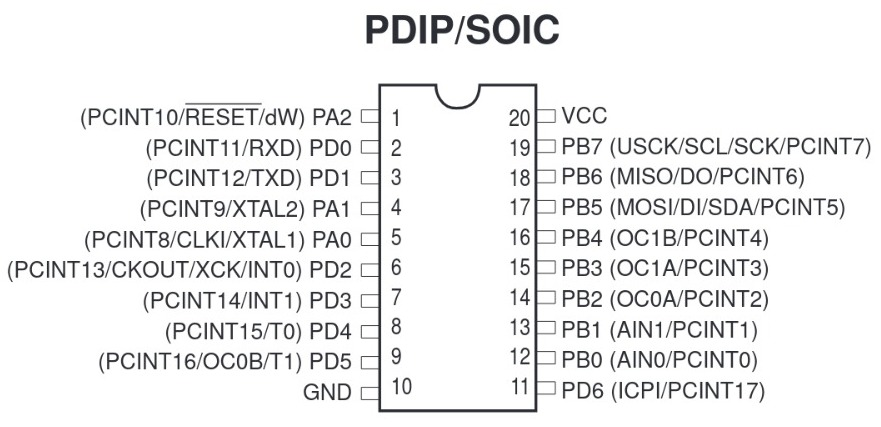
\includegraphics[scale=0.35]{images/Diagrama_pines.jpeg}
    \caption{Diagrama de pines\cite{Atmel2011}.}
    \label{fig:diagrama_pines}
\end{figure}

Para el presente laboratorio, se utilizaron los siguientes puertos: PB0, PB1, PB2, PB3, y PD2. 
\subsection*{Port B (PB7..PB0)}
Port B es un puerto de E/S bidireccional de 8 bits con resistencias pull-up internas que pueden ser seleccionadas para cada bit. Los búferes de salida de Port B presentan características de manejo simétricas, con alta capacidad tanto para hundir como para suministrar corriente. Cuando se utilizan como entradas, los pines de Port B que están externamente tirados a bajo generarán corriente si las resistencias pull-up están activadas. Los pines de Port B entran en estado de alta impedancia cuando se activa una condición de reinicio, incluso si el reloj no está en funcionamiento \cite{Atmel2011}.

\subsection*{Port D (PD6..PD0)}
Similar a Port B, Port D es un puerto de E/S bidireccional de 7 bits con resistencias pull-up internas seleccionables para cada bit. Los búferes de salida de Port D también tienen características simétricas de manejo de corriente. Al igual que con Port B, los pines de Port D que están externamente tirados a bajo generarán corriente si se activan las resistencias pull-up. Los pines de Port D también se ponen en estado de alta impedancia durante una condición de reinicio, incluso si el reloj no está funcionamiento \cite{Atmel2011}.

\begin{figure}[H]
    \centering
    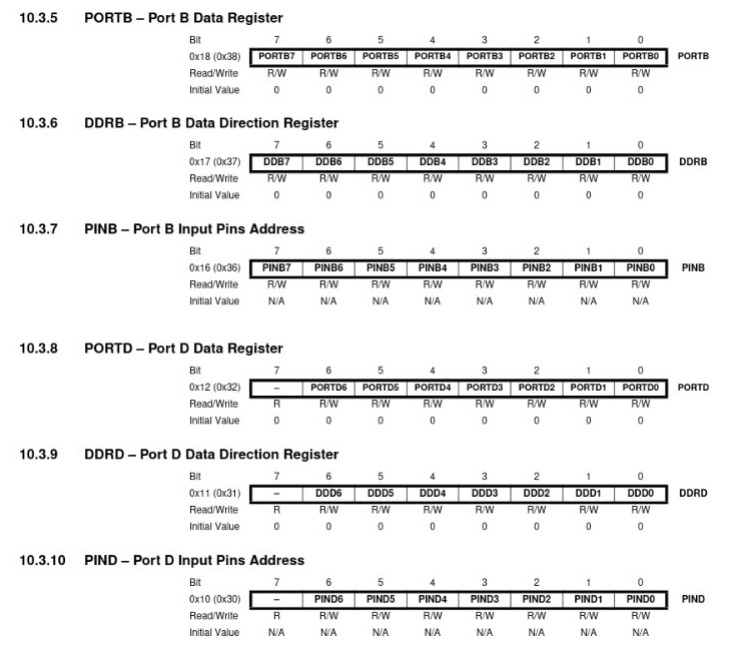
\includegraphics[scale=0.45]{images/puerto.jpeg}
    \caption{Descripción de pines\cite{Atmel2011}.}
    \label{fig:descripcion_pines}
\end{figure}

\subsection{Diagrama de bloques}
A continuación se presenta el diagrama de bloques del ATtiny4313:
\begin{figure}[H]
    \centering
    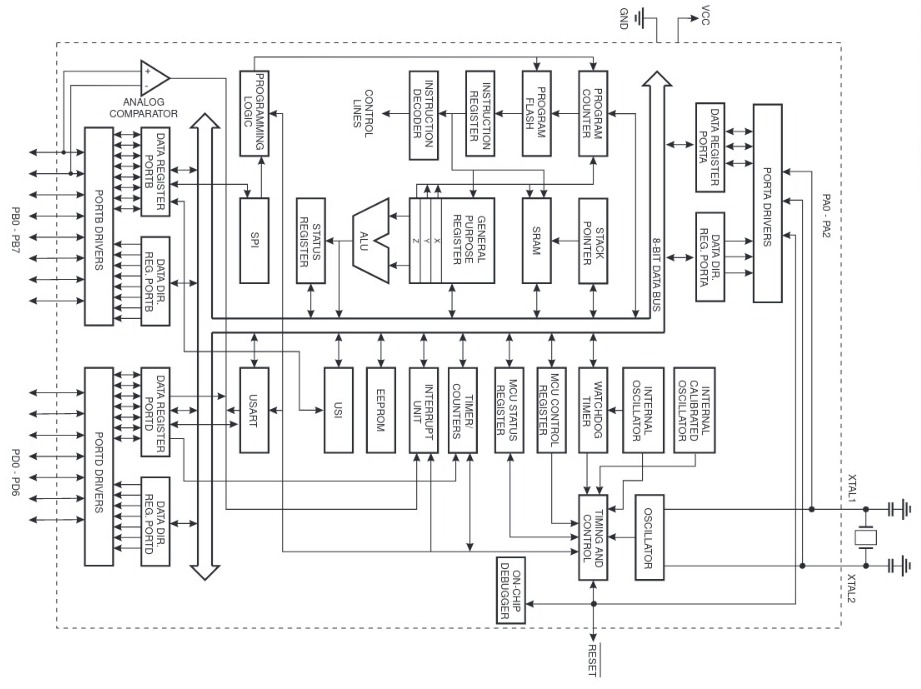
\includegraphics[angle=90, scale=0.4]{images/Diagra_bloques.jpeg}
    \caption{Diagrama de bloques \cite{Atmel2011}.}
    \label{fig:enter-label}
\end{figure}

\subsection{Interrupciones}

Las interrupciones son fundamentales para el funcionamiento eficiente de un microcontrolador. Cuando se activa una interrupción, la ejecución normal del programa se detiene temporalmente. El estado actual del programa, incluidas las variables y el contador de programa, se guarda en un bloque de memoria especial. Luego, el microcontrolador busca en este bloque para encontrar la Rutina de Servicio de Interrupción (ISR) correspondiente que necesita ser ejecutada \cite{Alley2011}.

Existen cuatro componentes clave en el mecanismo de interrupción:

\begin{enumerate}
  \item \textbf{Banderas de Interrupción:} Indican si ha ocurrido un evento de interrupción.
  \item \textbf{Bits de Habilitación de Interrupción:} Determinan si una interrupción específica será atendida automáticamente por el hardware.
  \item \textbf{Habilitación Global de Interrupciones:} Permite o impide que ocurran interrupciones en el sistema.
  \item \textbf{Rutina de Servicio de Interrupción (ISR):} Es el conjunto de instrucciones que se ejecuta cuando se produce una interrupción \cite{Alley2011}.
\end{enumerate}

La ejecución eficiente de las ISRs es crucial para el rendimiento del sistema, ya que evita pérdida de datos o comportamientos inesperados. Estas rutinas son responsables de guardar y restaurar el contexto del programa, permitiendo que el microcontrolador continúe su ejecución donde la dejó \cite{Alley2011}.


\subsection{Interrupciones Externas}
Las interrupciones externas son mecanismos que permiten a un microcontrolador detectar un cambio de estado en alguna de sus terminales de entrada, evitando así la necesidad de un sondeo continuo. Estas son especialmente útiles para monitorear estados de interruptores, botones, o sensores con salida a relevador. \cite{interrupciones}


\subsection{Configuración de las interrupciones}
Las interrupciones externas pueden configurarse para detectar un nivel bajo de voltaje o una transición en el flanco de subida o bajada. Sin embargo, la interrupción INT2 sólo puede activarse por flancos. Importante resaltar que estas interrupciones pueden generarse incluso cuando sus terminales respectivas son configuradas como salidas.

Las transiciones en INT0/INT1 requieren de una señal de reloj (clkI/O) para generar una interrupción. Esta señal de reloj es anulada en la mayoría de los modos de bajo consumo. Por otro lado, un nivel bajo en INT0/INT1 y las transiciones en INT2 no requieren de una señal de reloj, siendo eventos asíncronos y adecuados para despertar al microcontrolador en cualquier modo de reposo.\cite{interrupciones}
\begin{figure}[H]
    \centering
    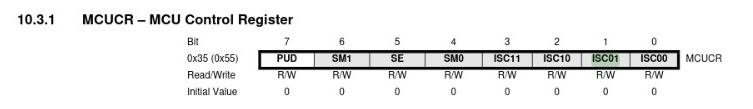
\includegraphics[scale=0.5]{images/MCUCR.jpeg}
    \caption{Configuración del MCUCR\cite{Atmel2011}.}
    \label{fig:enter-label}
\end{figure}
\begin{figure}[H]
    \centering
    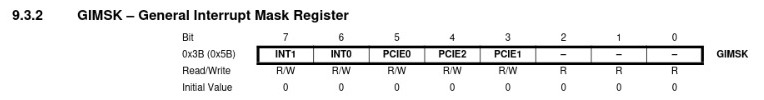
\includegraphics[scale=0.5]{images/GIMSK.jpeg}
    \caption{Configuración del GIMSK\cite{Atmel2011}.}
    \label{fig:enter-label}
\end{figure}
\begin{figure}[H]
    \centering
    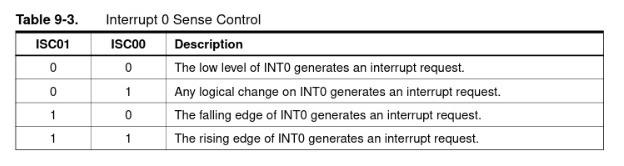
\includegraphics[scale=0.5]{images/int0.jpeg}
    \caption{Configuración del INT0\cite{Atmel2011}.}
    \label{fig:enter-label}
\end{figure}
\subsubsection{Configuraciones Específicas}

\paragraph{NT0: External Interrupt Request 0 Enable}
Cuando este bit y el bit I en el Registro de Estado (SREG) están activados, se habilita la interrupción externa en el pin INT0. Los bits de Control de Sentido de Interrupción (ISC01 y ISC00) en el Registro de Control de Interrupción Externa A (EICRA) determinan si la interrupción se activa en los bordes ascendentes y/o descendentes del pin INT0.

\paragraph{PUD: Pull-up Disable}
Al escribir un ``uno'' en este bit, se desactivan las resistencias \textit{pull-up} en los puertos de E/S.

\paragraph{ISC01, ISC00: Interrupt Sense Control 0 Bit 1 and Bit 0}
La Interrupción Externa 0 se activa por el pin externo INT0 si la bandera I del SREG y la máscara de interrupción correspondiente están establecidas.

\paragraph{Duración de la Señal para Interrupción}
Si se selecciona una interrupción de borde o de conmutación, los pulsos que duran más de un período de reloj generarán una interrupción. Los pulsos más cortos no garantizan la generación de una interrupción.

\subsection{Temporización en Microcontroladores ATMega}

\subsubsection{Importancia de la Temporización Precisa}

Mantener un tiempo preciso es crucial, especialmente en tareas que requieren mediciones exactas o en sistemas de navegación. Los temporizadores internos del microcontrolador permiten una gestión del tiempo altamente precisa, esencial para el control eficaz del sistema \cite{Alley2011}.

\subsubsection{Tipos de Temporizadores}

\paragraph{Temporizadores Internos}
Los microcontroladores ATMega8 y ATMega16 cuentan con temporizadores 0 y 1 que pueden funcionar como contadores de eventos externos.

\paragraph{Temporizadores Externos}
Están diseñados para funcionar con señales externas a través de los pines T0 y T1. Además, el temporizador 2 puede operar con un oscilador externo de 32.768 KHz.

\subsubsection{Modos de Operación}

\begin{itemize}
    \item \textbf{Modo 0:} Operación básica con eventos de desbordamiento.
    \item \textbf{Modos 1 y 3:} Utilizados para la generación de señales PWM.
    \item \textbf{Modo 2:} Permite limpiar el registro del temporizador en coincidencias específicas \cite{interrupciones}.
\end{itemize}

\subsubsection{Registros Importantes}
El temporizador 1 utiliza registros de 16 bits como TCNT1, OCR1A, OCR1B e ICR1 que son esenciales para su funcionamiento. Los registros TCCR1A y TCCR1B controlan el comportamiento del temporizador.
\begin{figure}[H]
    \centering
    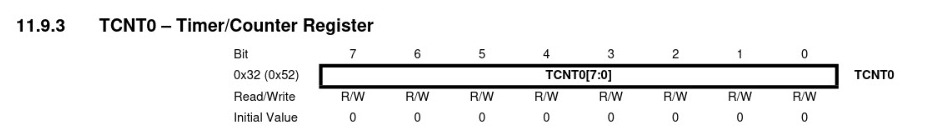
\includegraphics[scale=0.5]{images/TCNT0.jpeg}
    \caption{Configuración del TCNT0\cite{Atmel2011}.}
    \label{fig:enter-label}
\end{figure}

\begin{figure}[H]
    \centering
    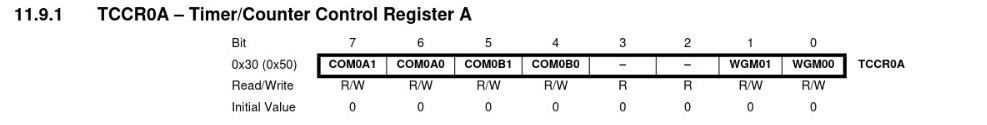
\includegraphics[scale=0.5]{images/TCCR0A_CL0.jpeg}
    \caption{Configuración del TCCR0A\cite{Atmel2011}.}
    \label{fig:enter-label}
\end{figure}
\begin{figure}[H]
    \centering
    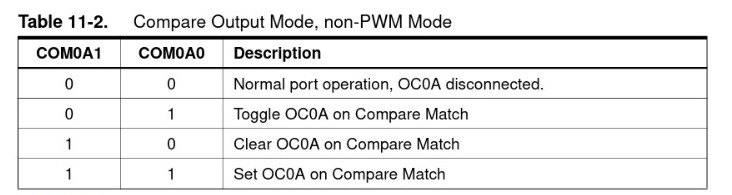
\includegraphics[scale=0.5]{images/COM0A.jpeg}
    \caption{Configuración del COMA0\cite{Atmel2011}.}
    \label{fig:enter-label}
\end{figure}
\begin{figure}[H]
    \centering
    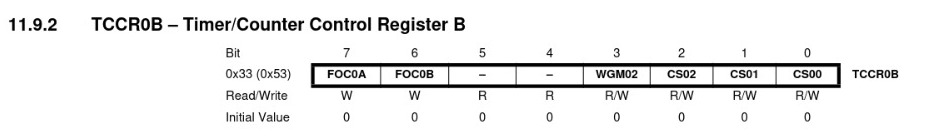
\includegraphics[scale=0.5]{images/TCCR0B.jpeg}
    \caption{Configuración del TCCR0B\cite{Atmel2011}.}
    \label{fig:enter-label}
\end{figure}
\begin{figure}[H]
    \centering
    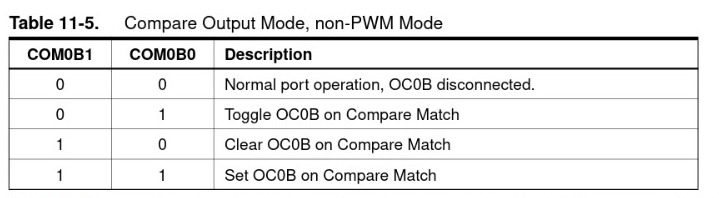
\includegraphics[scale=0.5]{images/COMB0.jpeg}
    \caption{Configuración del COMB0\cite{Atmel2011}.}
    \label{fig:enter-label}
\end{figure}
\subsubsection{Selección de la Fuente del Reloj}
Para el temporizador 0, la selección del reloj se controla con los bits CS0[2:0], y para el temporizador 1, con los bits CS1[2:0].








\newpage

\section{Desarrollo}

\subsection{Diseño}

Con el diseño implementado los dos botones al presionarse van a conectar el pin D2 a +5V, y  la corriente máxima que estos pines pueden proporcionar es de 40 mA. Sin embargo para asegurar el funcionamiento se limitó la corriente a 30 mA.

El valor de la tensión de los LEDs es de 2.0 V. Por lo tanto, utilizando Ley de Kirchhoff para calcular el valor de las resistencias para el caso de un solo LED:

\begin{equation}
    R = \frac{V_{DD} - V_{LED}}{I_{Max}} = \frac{5 - 2.0}{25 mA} =  120\Omega
\end{equation}

Tomando los valores en bodega de la escuela, se eligieron entonces resistencias de para cada uno de los LEDs de $120 \Omega$. Estas resistencias son de gran importancia para proteger los LEDs.

Además, es de suma importancia notar que un circuito RC se agregó para proteger de los efectos rebote a los botones. Se definió una resistencia de $10 K\Omega$ debido a que proporciona una corriente limitada a través del circuito para reducir el consumo de energía y la carga en la fuente de alimentación, seguidamente el capacitor de 10 nF ofrece un buen equilibrio entre filtrado y velocidad de respuesta de los botones. \cite{drmaker2014debouncing}

El tiempo que transcurre desde que se presiona el pulsador momentáneo hasta que el condensador se carga por completo se puede calcular utilizando la siguiente fórmula:

\begin{equation}
    Tiempo (segundos) = {Valor de R} \cdot {Capacidad del condensador}
\end{equation}

Calculando con los valores que se diseñaron para el circuito:

\begin{equation}
    Tiempo (segundos) = 10 K\Omega \cdot 10 nF
\end{equation}

\begin{equation}
    Tiempo (segundos) = 10 K\Omega \cdot 10 nF
\end{equation}

\begin{equation}
    Tiempo (segundos) = 0.1 s
\end{equation}

Este tiempo permite una respuesta lo suficientemente rápida para que el semáforo peatonal se active después de que el usuario presione el botón, y al mismo tiempo elimina de manera efectiva cualquier rebote en el interruptor

A nivel del código implementado, se puede mencionar que se agregaron ciertas características para poder optimizar el rendimiento y código. Entre ellas destacan el uso de macros para definir valores constantes y representar unidades de tiempo clave.

El uso de macros permiten asignar nombres significativos a valores numéricos, lo que hace que el código sea más legible, reutilizable y fácil de mantener. Además, las macros facilitan la modificación de estos valores en un solo lugar, lo que simplifica la adaptación del comportamiento del semáforo sin necesidad de buscar y cambiar cada instancia numérica en el código. Esta característica puede mejorar la escalabilidad del código, ya que cualquier ajuste necesario en los tiempos de cambio de estado o ciclos del temporizador se puede realizar de manera eficiente y precisa simplemente modificando las macros. 

Además otra implementación importante fue el uso de funciones \textit{inline} para funcionalidades como el parpadeo de las luces del semáforo y la gestión de las interrupciones.  ERste tipo de funciones se utilizan para evitar la sobrecarga de llamadas a funciones y, en su lugar, insertar directamente el código de la función en el lugar donde se invoca. Esto ahorra el tiempo y los recursos que normalmente se consumirían en la llamada y retorno de una función, lo que resulta en un código más rápido y eficiente en términos de rendimiento. \cite{microsoftInlineFunctions}

A continuación se muestran los costos de los componentes utilizados:

\begin{table}[h]
\centering
\begin{tabular}{|c|c|}
\hline
\textbf{Componente}     & \textbf{Precio} \\ \hline
ATtiny4313               & 583 colones    \\ \hline
Resistencia de 120 Ohms & 155 colones     \\ \hline
Botón                   & 150 colones     \\ \hline
Resistencia de 10 KOhms & 120 colones     \\ \hline
10 nF capacitor        & 325 colones     \\ \hline
LED Verde              & 310 colones     \\ \hline
LED Rojo              & 310 colones     \\ \hline
\end{tabular}
\caption{Precio de los componentes}
\label{tab:componentes}
\end{table}

\newpage
\subsection{Funcionalidad del diseño}
El circuito en el simulador se muestra de la siguiente manera:
\begin{figure}[H]
    \centering
    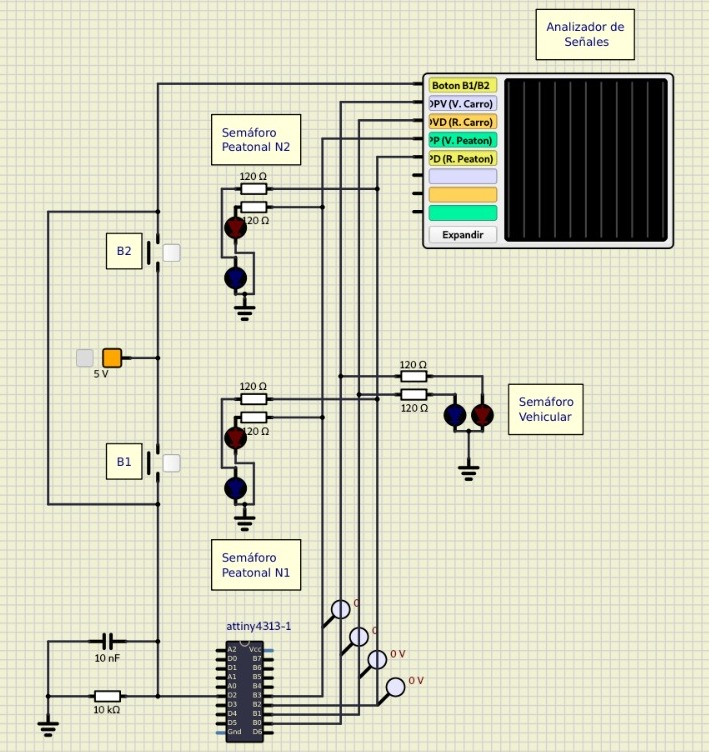
\includegraphics[scale=0.4]{images/Circuito_semaforo.jpeg}
    \caption{Diseño del circuito.}
    \label{fig:semaforo}
\end{figure}

Al poner a funcionar el simulador, se puede observar el estado inicial del semáforo a continuación. Puede notarse que en su estado inicial los semáforos peatonales se encuentran en rojo mientras que el semáforo vehicular en verse

\begin{figure}[H]
    \centering
    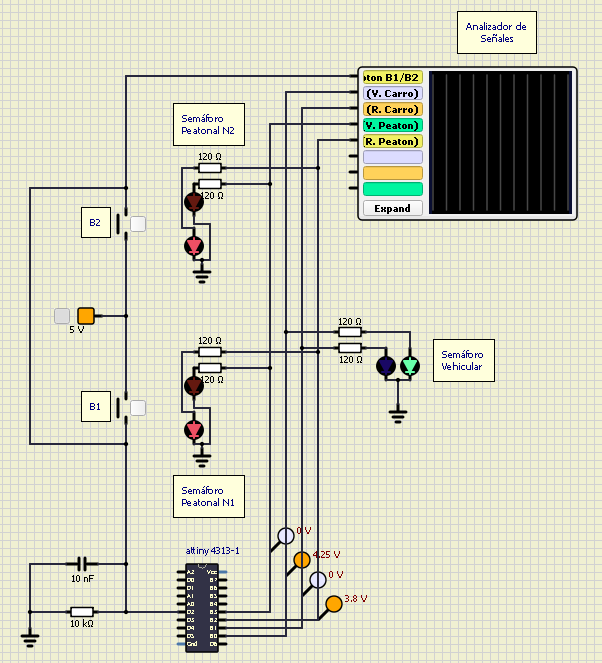
\includegraphics[scale=0.6]{images/uso1.png}
    \caption{Estado inicial del semáforo}
    \label{fig:semaforo2}
\end{figure}

Seguidamente, al presionar cualquiera de los dos botones se puede observar el semáforo peatonal en funcionamiento. El semáforo vehicular pasa a rojo mientras que los peatonales a verde


\begin{figure}[H]
    \centering
    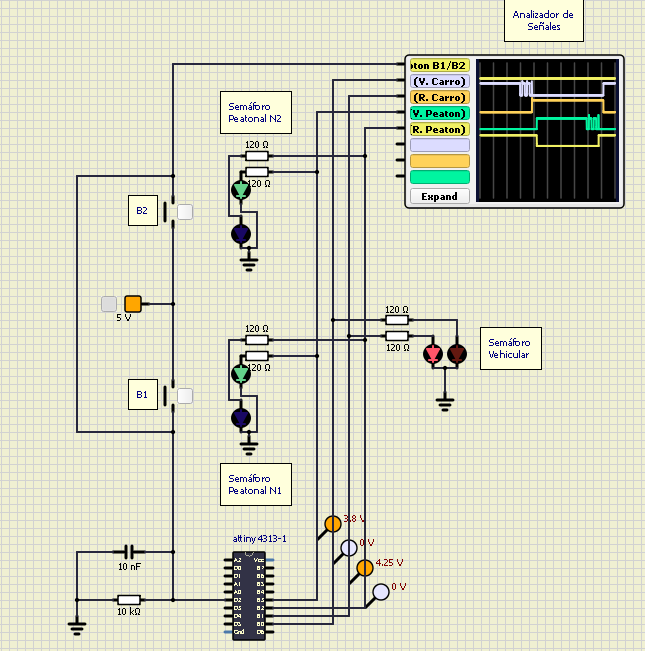
\includegraphics[scale=0.6]{images/uso2.png}
    \caption{Semáforos en funcionamiento}
    \label{fig:semaforo2}
\end{figure}

Finalmente, luego del tiempo definido para el funcionamiento de los semáforos peatonales, éstos vuelven a su estado inicial y el semáforo vehicular vuelve a estar en verde.

\begin{figure}[H]
    \centering
    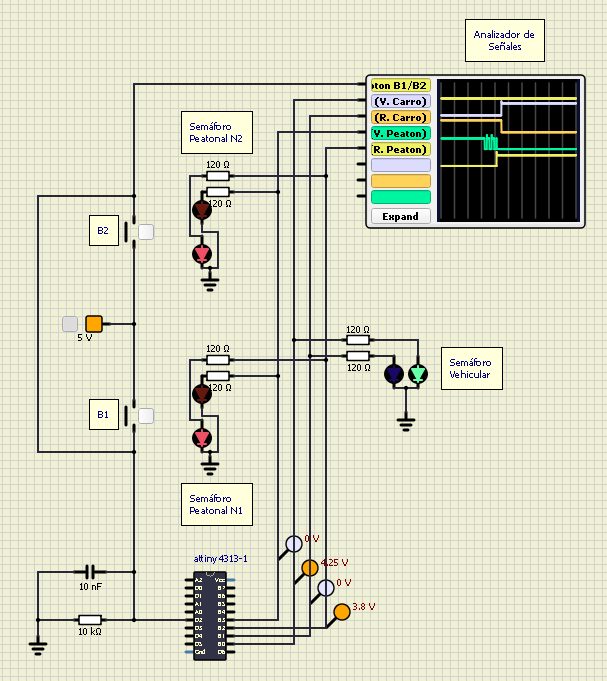
\includegraphics[scale=0.6]{images/uso3.png}
    \caption{Semáforos en funcionamiento}
    \label{fig:semaforo2}
\end{figure}

\newpage

\subsection{Diagrama de estados}
A continuación se presenta el diagrama de estados del proyecto:
\begin{figure}[H]
    \centering
    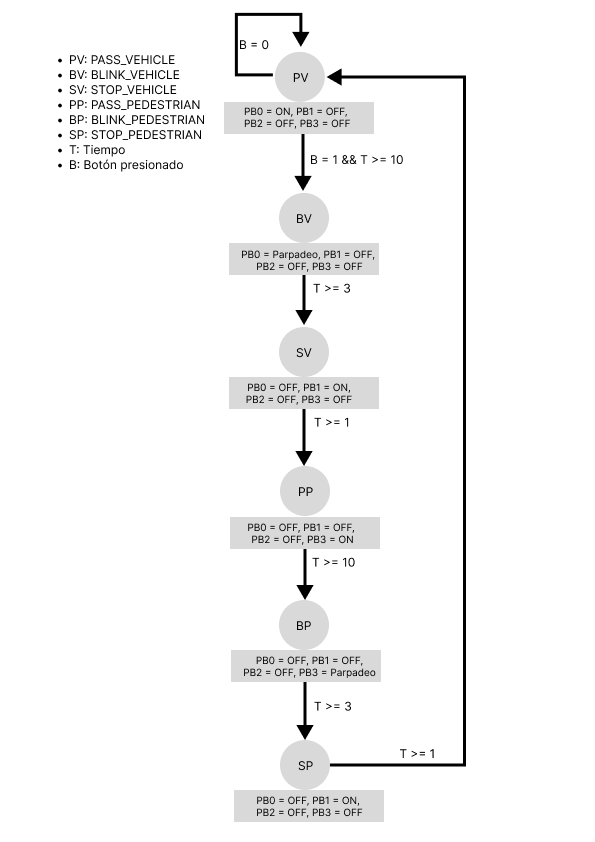
\includegraphics[scale=0.5]{images/Maquina de estados.png}
    \caption{Diagrama de estados.}
    \label{fig:diagrama_estados}
\end{figure}

\newpage
\subsection{Funcionalidad electrónica}
Se colocó un osciloscopio en las salidas de cada pin y en la entrada del botón para mostrar que los cambios en la tensión son los esperados. En la siguiente imagen se puede observar la lectura del osciloscopio.
\begin{figure}[H]
    \centering
    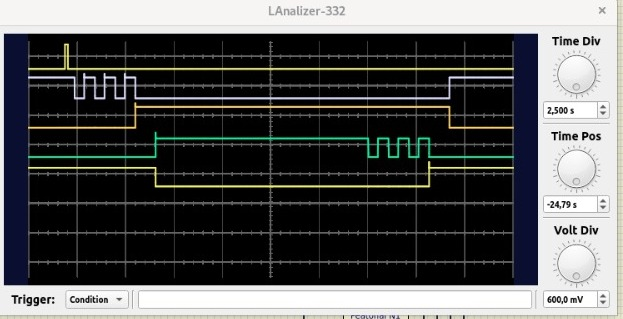
\includegraphics[scale=0.5]{images/Ondas_tiempo.jpeg}
    \caption{Lectura del osciloscopio.}
    \label{fig:diagrama_tiempo}
\end{figure}
Al inicio de las pruebas, todas las salidas se encontraban en un estado lógico bajo (`0'), cumpliendo con las expectativas iniciales. Del mismo modo, el botón de entrada también comenzó en un estado bajo. Cuando se presionó el botón, la señal asociada mostró un flanco ascendente, que activó una transición en la máquina de estados. Durante el experimento, las transiciones entre diferentes estados de las salidas se llevaron a cabo de manera coherente con la definición de la máquina de estados.

Además, se pudo verificar que cada estado se mantenía durante el período de tiempo especificado antes de avanzar al siguiente estado. Es importante destacar que durante las pruebas no se detectaron falsas transiciones ni ruido eléctrico que pudieran afectar la secuencia de estados. Esto indica que el sistema de ``debouncing'' para el botón funciona correctamente, y que la implementación de la máquina de estados funciona de la manera esperada.

\newpage

\section{Conclusiones y Recomendaciones}

\begin{itemize}
    \item  El diseño del circuito demostró ser eficaz y económico, optimizando la corriente de los LEDs y minimizando el ruido y los efectos de rebote en los botones. La selección de resistencias y el uso de un circuito RC contribuyeron al rendimiento óptimo del sistema.
    \item La funcionalidad de la máquina de estados se validó a través de pruebas con un osciloscopio, confirmándose que las transiciones de estado y la duración de los estados fueron las esperadas. No se observaron ruidos ni falsas transiciones.
    \item Se logró cumplir de manera correcta el diagrama de temporización propuesto en el enunciado del laboratorio
    \item Se logró construir un diseño funcional para el microcontrolador ATtiny4313, logrando así conocer sus funcionalidades y características.
\end{itemize}
 






\newpage
\bibliographystyle{IEEEtran}

\bibliography{bibliografia.bib}


\newpage

\section{Apéndices}

\begin{figure}[H]
    \centering
    \center
    \includegraphics[width=0.9\textwidth]{}
    \caption{Descripción arquitectónica. Creación propia.}
    \label{1}
\end{figure}

\end{document}